\section{Introduction}

  This document discusses the design and operation of the CFT Standard
  Assembler, introduced as the first and main implementation tool for
  writing CFT software. The CFT is a solid-state, 16-bit, microcoded
  architecture reminiscent, among others, of the DEC PDP-8. The
  computer incorporates a 16-bit word width with separate memory and
  input/output addressing spaces and a minimal, orthogonal instruction
  set that is still particularly versatile. The design includes
  separate internal (processor) and external (peripheral) buses and is
  extensible both via processor extensions and peripherals. The
  instruction set is extensible in the style of the PDP-8 using
  instruction-level aliasing (instruction macros) and assembler macros.

  The Standard Assembler is capable of producing optimised code for
  the CFT that takes advantage of the architecture's idiosyncrasies,
  and avoids the pitfalls of its many peculiarities.

  The Standard Assembler is a cross-compilation tool, written in
  Python to run on Unix and Unix-like computers. A possibly simplified
  version of the Standard Assembler is intended to be included as part
  of the CFT Forth Operating System, and possibly as a more
  full-featured stand-alone, native version.

\section{Architecture}

The Standard Assembler is a text-book multiple pass assembler with a
simple macro facility. It includes a ‘permanent’ symbol table with
macro definitions for the standard CFT instruction set as outlined in
the Programming Guide, in \cf{prog-guide}.

\subsection{The Cross Assembler}

The Cross Assembler is implemented in Python 2.6, but will probably run on
Python 2.4 or newer. It compiles the current version of ROM Forth in under two
seconds, which is quite acceptable performance. The choice of language also
makes it very easy to modify the assembler as necessary without much effort.

\section{Syntax}

Assembler syntax is simpler than the average assembler, to match the
simpler structure of the CFT.

Lines consisting of white space are ignored. Every other line must
contain one or more of the following:

\begin{itemize}
\item Comments.
\item Instructions.
\item Origin specifications.
\item Label declarations.
\item Assembler directives.
\item Macros.
\end{itemize}

\subsection{Comments}

Comments are introduced with the slash (\f{/}) or semicolon (\f{;})
characters. Conventional comments follow a C++-style (\f{//}) or Assembly
(\f{;;}) conventions, but this is not mandatory.

Any text after the first comment character is ignored, as expected.

\subsection{Instructions}

An instruction is one 16-bit value.

Each 16-bit instruction must be composed of one or more ‘fields’, each
separated by one or more spaces. All the values specified on a line get ORred
together to form an aggregate which is then assembled at the current address.

Each field must be one of the following things:

\begin{itemize}
  \item Symbols.
  \item Literal values.
  \item Expressions involving symbols and/or literal values.
\end{itemize}

\subsubsection{Symbols}

A symbol is a sequence of one or more symbol characters. The first character
must be an alphabetic character or an underscore (\f{\_}). Subsequent characters
may be alphanumeric or underscores.

Any symbol in the symbol table may be used as an instruction field, no matter
what its semantics are. Examples include opcodes such as \op{LOAD}, simple
field values such as \op{R}, labels, or other symbols.

Labels are treated specially if included in an instruction: the label's value (its
address), is masked by ANDing with value \hex{3FF}$_{16}$. In this format, a label
will fill the instruction's 10-bit operand field.

\subsubsection{Literal Values}

CFT Assembly supports 16-bit literal values in three formats:

\begin{description}
\item{\bfseries Decimal} A plain numerical value consisting of one to five digits
  between \f{0} and \f{9}.
\item{\bfseries Hexadecimal} The character \f{\&} or sequence \f{0x} followed by 1–4 digits,
  each between \f{0}–\f{9} or \f{A}–\f{F}. Lower case letters may also be used.
\item{\bfseries Binary} The character \f{\#} followed by 1–16 binary digits (\f{0} or
  \f{1}). To aid in defining readable bitfields, single quotes \f{'} and commas
  \f{,} are ignored. Additionally, dashes (\f{-}), periods (\f{.}) and
  underscores (\f{\_}) are treated as \f{0}. This allows bitfields to be
  defined as \f{\#----'0010}, clearly indicating ‘don't-care’ bits.
\end{description}

\subsubsection{Expressions}

Expressions perform simple arithmetic at assembly time. They come in three basic
formats:

\begin{description}

\item{\bfseries Current address}: \f{@}. A single at-sign (\f{@}) is replaced by the
  current address.

\item{\bfseries Relative address}: \f{@+{\bfseries value}} or \f{@-{\bfseries value}}. The value
  (which may be any parseable field value) is added or subtracted from the
  current address, and the result replaces the expression.

\item{\bfseries Full expression}: \f{@{\bfseries a op b}}. The operator {\bfseries op} is one of
  \f{+}, \f{-}, \f{*} (multiplication), \f{/} (division), \f{|} (bitwise OR),
  \f{\&} (bitwise AND), or \f{\char`\^} (bitwise XOR). There should {\em no space
    between the operator and the two operands}. For example, \f{@someLabel+\&80}
  is valid, while \f{@someLabel + \&80} is invalid. The two operands {\bfseries a} and
  {\bfseries b} are any parseable fields.

\end{description}

\subsection{Setting the Origin}

The origin is the next address to be assembled at. To set the origin, include a
literal value followed by a colon (\f{:}). For example, this sets the origin to
the CFT Reset vector at address \hex{FFF0}:

\begin{cftasmcode}
&FFF0:       ;; The CFT Reset Vector address
\end{cftasmcode}

\subsection{Labels}

Labels name a new symbol after the current address, so that the address can
then be referred to by name. Labels are essential in Assembly languages. They
simplify flow control and many other advanced tasks. A label is declared by
typing its name followed by a colon character (\f{:}). Multiple labels may be
set for the same address, one to a line. The origin may also be set. This is a
common idiom:

\begin{cftasmcode}
&FFF0:       ;; The CFT Reset Vector address
reset_vec:
reboot:
\end{cftasmcode}

Although declaring multiple labels for the same address is wasteful, it can
often lead to better readability.

\subsection{Directives}

A sequence of letters starting with a period (\f{.}) is a directive. Directives
assemble special values and modify the behaviour of the assembler. They are
similar in spirit to C preprocessor directives.



\subsubsection{Defining Arbitrary Symbols with \f{.equ}}

The \f{.equ} directive defines a new symbol with an arbitrary value. The syntax is:

\begin{cftasmcode}
.equ symbol value
\end{cftasmcode}

Any valid symbol may be named, and any parseable value may be used:
instruction, label, or literal. The most common uses of \f{.equ} are in
defining instructions or constants. The following definitions are actually part
of the permanent symbol table of the CFT Standard Assembler and cover the basic
instruction set:

\begin{cftasmcode}
.equ TRAP  &0000
.equ IOT   &1000
.equ LOAD  &2000
.equ STORE &3000
.equ IN    &4000
.equ OUT   &5000
.equ JMP   &6000
.equ JSR   &7000
.equ ADD   &8000
.equ AND   &9000
.equ OR    &A000
.equ XOR   &B000
.equ OP1   &C000
.equ OP2   &D000
.equ ISZ   &E000
.equ LIA   &F000

.equ R     &0400
.equ I     &0800
\end{cftasmcode}

After definition, symbols may be used wherever parseable values may be used,
including in subsequent \f{.equ definitions}:

\begin{cftasmcode}
.equ LIA   &F000
.equ LI    LIA  R   ; &F000 | &0400
\end{cftasmcode}

This is exactly how the assembler defines the standard instruction macros, of
which \op{LI} is one.



\subsubsection{Declaring Registers with \f{.reg}}

The \f{.reg} directive works like the \f{.equ} directive, with one exception:
it declares a location in memory (usually Page 0) to be used as a register. For
example:

\begin{cftasmcode}
.reg  R0   R &10
.reg  R1   R &11
.reg  R2   R &12
.reg  R3   R &13

.reg  I0   R &80 ; Autoincrement registers
.reg  I1   R &81
.reg  I2   R &82
.reg  I3   R &83
\end{cftasmcode}

The difference between \f{.equ} and \f{.reg} is mainly one of semantics:
\f{.equ} can define such diverse entities as I/O locations, addresses, labels,
constants, flags, instructions, bit masks, et cetera — this sometimes makes it
difficult to divine the purpose of a symbol, even if good coding practices are
used. In contrast, \f{.reg} is meant only for register declaration, and this is
reflected in the various output files (map, symbol tables and graphical maps).

It is almost always useful to define registers with the \asm{R} field
set, as is done in the example above. This makes it simpler to
reference the registers without having to use \asm{R}, and reduces
bugs caused by the \asm{R} left out\footnote{Empirical evidence has
  shown that this is a very common and potentially insidious problem
  with CFT Assembly code.}.

\subsubsection{Including Assembly Files with \f{.include}}

The \f{.include} directive instructs the Assembler to read, process and
assemble an external file. It is used like this:

\begin{cftasmcode}
.include "some_file.asm"
\end{cftasmcode}

This may be used to break large programs into manageable, semantically distinct
blocks, or to allow libraries of definitions or code to be defined and shared
among programs.



\subsubsection{Assembling Arbitrary Data with \f{.word}}

The \f{.word} directive assembles an arbitrary word at the current
address. Some examples of its syntax:

\begin{cftasmcode}
.word some_label  ; label address
.word @           ; assemble current address
.word @+10        ; current address + 10
.word STORE       ; assemble an instruction
.word 1 #10 &4 8  ; assemble decimal value 15
\end{cftasmcode}

Any parseable value may be assembled using the \f{.word} directive, including
instructions.

Unlike plain instruction assembly, \f{.word} does not treat labels specially:
when assembling the value of a label in an instruction, only the lower 10 bits
are used. With \f{.word}, all 16 bits are used. This makes \f{.word} invaluable
in generating vector tables and aiding in indirection.



\subsubsection{Filling Regions with a Value with \f{.fill}}

The \f{.fill} directive assembles a value and uses it to fill a block in the
object code starting with the current address. It syntax is:

\begin{cftasmcode}
.fill COUNT VALUE
\end{cftasmcode}

The \op{COUNT} must be a literal value. The \op{VALUE} may be any parseable
value, including symbols and instructions. For example, to assemble 50 copies
of the value \hex{0000}:

\begin{cftasmcode}
.fill 50 &0000
\end{cftasmcode}

To fill a region with an instruction:

\begin{cftasmcode}
.fill &10 HALT
\end{cftasmcode}

Please note that the value is calculated {\em once}, so relative addressing and
expressions will not have the expected effect. The following directive will
assemble 10 copies of the instruction \op{JMP 0}, {\em not\/} a chain of jumps
with increasing addresses, despite the use of \op{@}.

\begin{cftasmcode}
&1000:  .fill 10 JMP @
\end{cftasmcode}



\subsubsection{Declaring Register Arrays with \f{.regfill}}

Sometimes blocks of registers need to be declared — for example, to account for
a memory-mapped device with arrays of mapped values (such as a
framebuffer). The \op{.regfill} directive is used for that. It works exactly
like \op{.fill}, but also marks the filled area as a register array.



\subsubsection{Unpacked Strings with \f{.str}}

An unpacked string is a block of memory which represents character text. Each
character occupies an entire word and has a 16-bit range. Unpacked strings can
contain Unicode characters in UCS-2 or UTF-16 encodings. They can, of course,
contain ASCII characters as well. Since the CFT is a word-addressed machine,
these are the easiest strings for the computer to handle.

The \f{.str} directive assembles a string of values starting at the current
address:

\begin{cftasmcode}
.str "Hello World!" 10 0
\end{cftasmcode}

Character data are enclosed in double quotes, but \f{.str} can handle multiple
fields including any parseable value from literals to instructions (of course,
the utility of assembling instructions with \f{.str} is very limited). This may
be used to embed non-printable values (and double quotes) in strings. In the
example above, there is an ASCII 10 (line feed, return or new line) after the
exclamation point, followed by an ASCII 0 (NUL), which is conventionally used
to terminate variable-length strings.

\subsubsection{Arbitrary Data Blocks with \f{.data}}

The \f{.data} directive works in exactly the same way as the \f{.str}
directive. They differ only in semantics. The latter is expected to be used for
character strings, the former for arbitrary data, which {\em does\/} include
character data. An example:

\begin{cftasmcode}
.data &1234 &5678 &9abc &def0 "ABCDEFG"
\end{cftasmcode}

\subsubsection{Negative-Terminated Strings with \f{.strn}}

Negative-terminated strings are unpacked strings in which end of string is
indicated by setting bit 15 on the last character. This allows characters with
codepoints between 0–32,767 to be used. If the upper 32,768 codepoints are not
necessary, this representation saves one word per string. The \f{.strn}
directive works in exactly the same way as the \f{.str} directive:

\begin{cftasmcode}
.strn "Hello World!" 10
\end{cftasmcode}

However, the last character of the string will be ORred with the value
\hex{8000}, to produce this sequence of values in memory:

\begin{intrcode}
0048 0065 006c 006c 006f 0020 0057 006f
0072 006c 0064 0021 800a
\end{intrcode}

Note that the terminating null conventionally added to the end of \f{.str}
directives is unnecessary here.



\subsubsection{Packed Strings with \f{.strp}}
\label{sec:asm-pstring}

Packed strings are the most compact means of encoding strings of 8-bit
characters (or Unicode characters encoded in UTF-8) on the CFT
architecture. Two characters are assembled per word, with the first character
in the lower eight bits. This byte order mirrors the way little-endian
byte-addressable machines work when dealing with strings, which makes CFT
binary files easier to examine on other computers\footnote{That is, the
  majority of computers owned by the author.}. The syntax of the \f{.strp} is
identical to that of \f{.str}:

\begin{cftasmcode}
.strp "Hello World!" 10 0
\end{cftasmcode}

This will generate the following sequence of words:

\begin{intrcode}
6548 6c6c 206f 6f57 6c72 2164 000a
\end{intrcode}

Obviously, strings with odd length will have 8 unused bits in the last
position. This string is even-length (the terminating null counts). This,
however, still makes the string much more compact than the equivalent unpacked
string. Unfortunately, it also makes it more difficult to handle in machine
code. CFT Forth makes heavy use of packed strings to keep the size of the
dictionary down.



\subsubsection{Skipping to the Next Page with \f{.page}}

Since CFT is unable to reference ‘far’ addresses (across page boundaries)
without indirection, the vast majority of loops must not cross page
boundaries. Take this trivial loop, for example:

\begin{cftasmcode}
        LI 50
        NEG
        STORE R &10
loop:   ISZ R &10
        JMP loop
\end{cftasmcode}

Since addresses in instructions are 10 bits long, only the lower 10 bits of the
address of label \op{loop} are assembled in the \op{JMP} instruction. The upper
six bits are populated using the upper six bits of the current address
(i.e. the page). Now, assume \op{loop} is at address \hex{1FFF}. This places
\op{JMP} at address \hex{2000}, crossing a page boundary. The address in
\op{JMP} is still \hex{3FF} (the lower 10 bits of \hex{1FFF}, the address of
\op{loop}). However, the upper six bits are no longer \hex{1C00} (shifted) —
they are now \hex{2000}. Thus, the machine will jump to address \hex{23FF} and
the loop will fail. This is a problem common to all paged instruction sets.

The CFT Standard Assembler refuses to fix this automatically, instead producing a warning:

\begin{intrcode}
source.asm:5:warning: Label 'loop' on page 1c00,
  but page 2000 accessed instead.
\end{intrcode}

To solve this issue, code must be rearranged so that the loop does not cross
the page boundary. While developing, the easiest way to do this is to force
crossing the page boundary by changing the origin. This is the purpose of the
\f{.page} directive: it changes the origin to the first address of the next
page.

Please note that this should not be done inside subroutines, since a block of
unassembled values will be introduced. It should, instead, be placed just
before the entry point of a subroutine preceding the problem addresses.

The syntax is trivial:

\begin{cftasmcode}
.page
\end{cftasmcode}

A common issue is for \f{.page} directives to be left in the code while
developing, leading to large amounts of unused space. The assembler will let
the programmer know about potential cases of unnecessary \f{.page} directives
by issuing a warning:

\begin{intrcode}
file.asm:924:warning: .page generated 865 words of slack space.
\end{intrcode}

In such case, it is standard practice to comment out the directive (since
further coding is likely to push the problem code across another page boundary,
so the \f{.page} could be needed again).



\subsection{Instruction Macros}

The CFT instruction set contains sixteen main instructions, of which two allow
combinations of dozens of minor operations. Because of both the small size of
the instruction set and its versatility, many new instructions a programmer
would expect to have may be formed as combinations (or special cases) of other
instructions that are still technically one instruction.

For example, the CFT instruction set lacks shifts, but has rolls which rotate
the bits in the \AC{} register through the single-bit \Lreg{} register. An
unsigned shift may be implemented by clearing \Lreg{} before rolling, so that
the new instruction \op{SBL} is implemented by \op{OP1 CLL RBL}.

These instruction macros are defined inside the Standard Assembler using the
\f{.equ} directive and can be treated as {\em single} instructions. For example:

\begin{cftasmcode}
.equ   SBL   OP1 CLL RBL   ; Shift bit left
.equ   SBR   OP1 CLL RBR   ; Shift bit right
\end{cftasmcode}



\subsection{Assembler Macros}

In addition to defining instruction macros which expand the CFT {\em
  instruction set}, the Assembler also provides Assembler Macros which expand
the {\em assembly language}. Unlike instruction macros, assembler macros can
incorporate multiple instructions and are parametric. They are invaluable in
simplifying assembly listings and maintaining consistency.

\subsubsection{Defining New Macros}

New macros are defined with the \f{.macro} and \f{.end} directives. This is an
example of an ‘add with carry’ macro to provide addition with carry-in (which
cannot be implemented as a single CFT instruction):

\begin{cftasmcode}
.macro ADC (addr)
    OP1 IFL INC    ; Inc AC if L is set
    ADD %addr
.end
\end{cftasmcode}

The name of the macro is \op{ADC}, and this is how it will be called after its
definition. It accepts a single argument named \op{addr}. Please note that
macros without parameters {\em still} require the open and closing parentheses,
in the same way as C function definitions do.

Multiple arguments may be specified, separated by commas.

The code between \f{.macro} and \f{.end} is not assembled immediately — it is
stored for inclusion later.

Argument values may be used by prefixing their names with \f{\%}, hence the use
of \f{\%addr}.

\subsubsection{Calling Macros}

To call the \f{ADC()} macro, use this syntax:

\begin{cftasmcode}
ADC(R &10)
\end{cftasmcode}

The presence of the parentheses in an instruction line trigger a search for the
macro nominated before the opening parentheses. White space may be used between
the name and open parenthesis, but is not recommended to keep the code compact
and allow longer macro names.

Multiple argument values must be separated by commas.

The same number of values must be specified as there are arguments in the macro
definition. Macro calls may not have variable arguments lists. In the case of
\f{ADC}, exactly one argument may be specified. The value of the argument
depends on its use in the macro definition, but the vast majority are parseable
values.

\subsubsection{Unique Labels}

If a macro contains loops or declares labels and the macro is expanded multiple
times, some or all of those labels may need to be made unique. This may be done
by including the magic argument \f{\%\_} in any label names:

\begin{cftasmcode}
.macro MINILOOP(n, loopreg, op)
    LI %n
    NEG
    STORE %loopreg
miniloop%_:
    %op
    ISZ %loopreg
    JMP miniloop%_
.end
\end{cftasmcode}

Note the idiom of appending \f{\%\_} to the labels. The \f{\%\_} argument will
expand to a number to each macro expansion, making the label unique across the
assembly process. This is generally not recommended. If loops are necessary, it
may be better to implement them as subroutines.


\subsubsection{Advanced Use Patterns}

Because of the generality of the macro mechanism, some commonly performed
advanced tasks may be simplified greatly by using macros. A common use pattern
is to \asm{LOAD} a value, operate on it, then \asm{STORE} it back. This is a
side-effect of having a single-operand instruction set. Using advanced macros,
CFT Assembly may be expanded from single-operand to a more compact, more
readable three-operand format:

\begin{cftasmcode}
.macro RMOV(tgt, src) ; Move one register to another
	LOAD %src
	STORE %tgt
.end

.macro _RAPPLY(op, tgt, a, b) ; Apply an operation to a register
	LOAD %a
	%op %b
	STORE %tgt
.end

.macro RADD(tgt, a, b)
	_RAPPLY(ADD, %tgt, %a, %b)
.end

.macro RAND(tgt, a, b)
	_RAPPLY(AND, %tgt, %a, %b)
.end
\end{cftasmcode}

This now allows code to be written in this two- and three-operand idiom, very
reminiscent of RISC Assemblies like that of the MIPS Rx000.

\begin{cftasmcode}
        RMOV(R1, R3)            ;; mem[R1] = mem[R3]
        RMOV(R2, R4)            ;; mem[R2] = mem[R4]
        RADD(R0, R1, R2)        ;; mem[R0] = mem[R1] + mem[R2]
        RAND(R5, R1, R2)        ;; mem[R5] = mem[R1] & mem[R2]
\end{cftasmcode}

This is significantly more readable than the equivalent code without macros:

\begin{cftasmcode}
        LOAD R3                 ;; mem[R1] = mem[R3]
        STORE R1
        LOAD R4                 ;; mem[R2] = mem[R4]
        STORE R2
        LOAD R1                 ;; mem[R1] = mem[R2] + mem[R3]b
        ADD R2
        STORE R0
        LOAD R1                 ;; mem[R1] = mem[R2] + mem[R3]b
        AND R2
        STORE R5
\end{cftasmcode}


\section{Features}

The CFT Assembler includes various features to aid in debugging the object
code, simulating its execution in the CFT Emulator, as well as locating and
fixing issues with the Assembler itself.

















\begin{figure}
\begin{cftasmcode}
&c000: &0cf7 ;         .word &0cf7             ; Magic (CFT)
&c001: &c000 ;         .word @-1               ; Origin addr.
&c002: &0001 ;         .word 1                 ; Number of programs
&c003: &0000 ;         .word 0                 ; Reserved
&c004:       ;         .strp "CFT Forth ROM 0.1            " 0
&c004: &4643 ; "CF" (U+0043 U+0046)
&c005: &2054 ; "T " (U+0054 U+0020)
&c006: &6f46 ; "Fo" (U+0046 U+006f)
&c007: &7472 ; "rt" (U+0072 U+0074)
&c008: &2068 ; "h " (U+0068 U+0020)
&c009: &4f52 ; "RO" (U+0052 U+004f)
&c00a: &204d ; "M " (U+004d U+0020)
&c00b: &2e30 ; "0." (U+0030 U+002e)
&c00c: &2031 ; "1 " (U+0031 U+0020)
&c00d: &2020 ; "  " (U+0020 U+0020)
&c00e: &2020 ; "  " (U+0020 U+0020)
&c00f: &2020 ; "  " (U+0020 U+0020)
&c010: &2020 ; "  " (U+0020 U+0020)
&c011: &2020 ; "  " (U+0020 U+0020)
&c012: &0020 ; " ." (U+0020 U+0000)
&c013: &c014 ;         .word init              ; Entry point
&c014: &70a1 ;         JSR init_tables
&c015: &707b ;         JSR init_serial
&c016: &707f ;         JSR init_isr
\end{cftasmcode}
\caption[Preprocessed Assembly Output Example]{\label{fig:pasm-file} Example of
  a Preprocessed Assembly file (\texttt{.pasm}). It shows the beginning of the
  ROM Forth, with ROM boilerplate and the beginning of the code. The file can
  be fed back to the assembler: it contains address/assembled value pairs with
  corresponding code in comments.}
\end{figure}


\begin{figure}
\begin{intrcode}
v_TFORTH                  0200  _generated_tables.asm:16
_vector_table             0200  forth.asm:66
v__NEXT                   0201  _generated_tables.asm:17
v__doLIST                 0202  _generated_tables.asm:18
v__doCOL                  0203  _generated_tables.asm:19
v__doVAR                  0204  _generated_tables.asm:20
v__doCONST                0205  _generated_tables.asm:21
v__do2CONST               0206  _generated_tables.asm:22
v__doUSER                 0207  _generated_tables.asm:23
v__doVOC                  0208  _generated_tables.asm:24
v__doDOES                 0209  _generated_tables.asm:25
v__EXIT                   020a  _generated_tables.asm:26
_vector_table_end         020b  forth.asm:71
_does_table               020b  forth.asm:72
_does_table_end           0300  forth.asm:74
UP0                       0300  forth.asm:211
user_area                 0400  forth.asm:224
data_stack                0500  forth.asm:227
\end{intrcode}
\caption[Map File Example]{\label{fig:map-file} Example of a Map File
  (\texttt{.map}). It shows labels, their values and the location of their
  definition in the source code.}
\end{figure}

\begin{figure}
\begin{intrcode}
Name                      Val   Type    Defined in
----------------------------------------------------------
PANEL                     0408  symbol  ../asm/io.asm:4
LSR                       4408  symbol  ../asm/io.asm:5
LDSR                      4409  symbol  ../asm/io.asm:6
SOR                       540a  symbol  ../asm/io.asm:7
HALT                      540f  symbol  ../asm/io.asm:8
TTY0                      0460  symbol  ../asm/io.asm:17
TTY1                      0468  symbol  ../asm/io.asm:18
TTY2                      0470  symbol  ../asm/io.asm:19
TTY3                      0478  symbol  ../asm/io.asm:20
TTYRHR                    0000  symbol  ../asm/io.asm:27
TTYTHR                    0000  symbol  ../asm/io.asm:28
\end{intrcode}
\caption[Symbol File Example]{\label{fig:sym-file} Example of a Symbol File
  (\texttt{.sym}). It tabulates the entire symbol table with name, value,
  symbol type, and location of definition.}
\end{figure}



\section{Output}

At the end of the assembly process, the Assembler outputs a number of files,
most of which are both machine and human-readable.

\subsection{Object Files}

The object code generated by the assembler is a pure binary file with no
headers or magic numbers. They are files containing 16-bit words, one per
assembled value, starting at the start address specified to the assembler, and
ending at the end address, also as specified to the assembler.

\subsection{Verilog List Files}

To help using the code with the Verilog-based hardware verification suite, the
Assembler also outputs a pair of {\ttfamily .list} files with suffixes {\ttfamily -00.list}
(low order bits) and {\ttfamily -01.list} (high order bits). These are encoded in
Verilog-compatible human-readable binary and represent low and high ROM images
for the assembled code.

\subsection{The Map File}

The map file is generated with a {\ttfamily .map} suffix, and contains a map of the
labels declared in the source code. It contains three columns:

\begin{enumerate}
\item Label Name.
\item Address in zero-padded hexadecimal.
\item Location of definition in the source code in {\ttfamily filename:line} format.
\end{enumerate}

Part of the map file for ROM Forth is shown in~\fcf{fig:map-file}.

\subsection{The Symbol Table File}

Similar to the map file, this file (with a {\ttfamily .sym} suffix) contains a dump
of the entire symbol table, not just labels. It has a two-line header for human
readability, and contains lines arranged in four columns:

\begin{enumerate}
\item Symbol Name.
\item Value in zero-padded hexadecimal.
\item Symbol type:
  \begin{itemize}
  \item \f{symbol}: a symbol declared by \f{.equ}.
  \item \f{label}: a label.
  \item \f{register}: a register declared by \f{.reg} or \f{.regfill}.
  \end{itemize}
  \item The location of the symbol definition in the source code in {\ttfamily filename:line} format.
\end{enumerate}

A partial example of a symbol file for ROM Forth is shown in~\fcf{fig:sym-file}.

\subsection{The Preprocessed Assembly File}

Files with a {\ttfamily .pasm} suffix are ‘preprocessed assembly’ files. They contain
a digested form of the program, which is valid input to the CFT assembler, but
much less human-readable. Each line contains an explicit address followed by
the exact hexadecimal value at that address. The original assembly line leading
to that value follows as a comment. Strings and other multi-word directives are
expanded to show what is assembled. Include directives and macros are
expanded. No labels or other symbols are used (but remain in the
comments). Lines without assembled values are excluded. For example, label
declarations on their own lines will be left out.

These files may be used as a kind of assembly-annotated hex dump of the object
file, and are also used by the CFT emulator to print out the assembly source it
is executing.

Part of the preprocessed output for ROM Forth is shown in~\fcf{fig:pasm-file}.


\subsection{Graphical Memory Maps}

These are bitmap images useful in visualising the memory map of the program,
and the layout of the object file. They are output in the {\ttfamily .xpm} format,
which {\em is\/} human readable, although these files are too large for a human
to visualise without software. Like all {\ttfamily .xpm} files, this file is also
valid C code. It may be viewed with most image viewers or converted to a binary
bitmap file to save space.

The memory map displays the 65,536 word address space of the CFT as an array of
256×256 locations, with rows representing higher order bits of the address, so
that address \hex{0000} is at the upper left, and address \hex{FFFF} is at the
lower right.

Grey represents unused locations. Black represents slack space left by
\f{.page} directives. Magenta areas are those declared with \f{.reg}, and those
are expected to be at or near the top, on page 0. Red represents assembled
instructions. Orange represents packed strings. Green is for unpacked
strings. Blue represents \f{.word} values, and cyan marks \f{.fill} areas.

\begin{figure}[t]
\centering
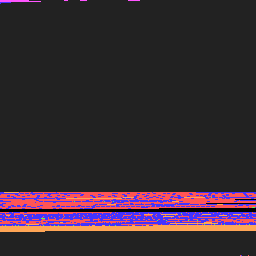
\includegraphics[width=0.5\columnwidth]{figs/forth.png}\\
\caption{\label{fig-graphical-map}A graphical memory map of a CFT assembly program.}
\end{figure}
